\documentclass[a4paper,10pt]{article}
\usepackage[utf8]{inputenc}
\usepackage{amsmath}
\usepackage{fullpage}
\usepackage{hyperref}
\usepackage{graphicx}
\usepackage{listings}
\usepackage{color}

\definecolor{mygreen}{rgb}{0,0.6,0}
\definecolor{mygray}{rgb}{0.5,0.5,0.5}
\definecolor{mymauve}{rgb}{0.58,0,0.82}

\lstset{ 
  backgroundcolor=\color{white},   % choose the background color; you must add \usepackage{color} or \usepackage{xcolor}; should come as last argument
  basicstyle=\footnotesize,        % the size of the fonts that are used for the code
  breakatwhitespace=false,         % sets if automatic breaks should only happen at whitespace
  breaklines=true,                 % sets automatic line breaking
  captionpos=b,                    % sets the caption-position to bottom
  commentstyle=\color{mygreen},    % comment style
  deletekeywords={...},            % if you want to delete keywords from the given language
  escapeinside={\%*}{*)},          % if you want to add LaTeX within your code
  extendedchars=true,              % lets you use non-ASCII characters; for 8-bits encodings only, does not work with UTF-8
  firstnumber=1,                   % start line enumeration with line 1000
  frame=single,	                   % adds a frame around the code
  keepspaces=true,                 % keeps spaces in text, useful for keeping indentation of code (possibly needs columns=flexible)
  keywordstyle=\color{blue},       % keyword style
  language=Python,                 % the language of the code
  morekeywords={*,...},            % if you want to add more keywords to the set
  numbers=left,                    % where to put the line-numbers; possible values are (none, left, right)
  numbersep=5pt,                   % how far the line-numbers are from the code
  numberstyle=\tiny\color{mygray}, % the style that is used for the line-numbers
  rulecolor=\color{black},         % if not set, the frame-color may be changed on line-breaks within not-black text (e.g. comments (green here))
  showspaces=false,                % show spaces everywhere adding particular underscores; it overrides 'showstringspaces'
  showstringspaces=false,          % underline spaces within strings only
  showtabs=false,                  % show tabs within strings adding particular underscores
  stepnumber=1,                    % the step between two line-numbers. If it's 1, each line will be numbered
  stringstyle=\color{mymauve},     % string literal style
  tabsize=4,	                   % sets default tabsize to 2 spaces
  title=\lstname                   % show the filename of files included with \lstinputlisting; also try caption instead of title
}


\renewenvironment{abstract}
 { \vspace*{0.3cm} \textbf{\abstractname} \vspace{0.1cm} \\ \ignorespaces}
 {\par\medskip \vspace{0.1cm}}

\setlength{\parindent}{0em}

\setlength{\textheight}{25.7cm}
\setlength{\textwidth}{18cm}
\setlength{\unitlength}{1mm}
\setlength{\topskip}{2truecm}

\topmargin 260mm \advance \topmargin -\textheight
\divide \topmargin by 2 \advance \topmargin -1in
\headheight 0pt \headsep 0pt \leftmargin 210mm \advance
\leftmargin -\textwidth
\divide \leftmargin by 2 \advance \leftmargin -1in
\oddsidemargin \leftmargin \evensidemargin \leftmargin
\parindent=0pt
\frenchspacing


%opening
\title{\textbf{Numerical Recipes for Astrophysics \\ Solutions hand-in assignment-2}}
\author{Luther Algra - s1633376}

\begin{document}

\maketitle

\hrule
\begin{abstract}
The current document contains the solutions for the second hand-in assignment of Numerical Recipes. Each main question 1, 2, 3, ..., 7 is given its own section and contains a subsection for each sub-question (1.a, 1.b, ..., 1.f). A main question always ends with a final subsection that contains two segments of code. The first segment contains the full code of the program that executes the sub-questions. The second segment contains the shared modules (if any) used by the sub-question. A sub-question itself always starts with a short summary of the question that needs to be answered followed by an explanation of how the problem is solved. Next, the code and its output are provided. Finally the output is discussed if relevant. 


\end{abstract}
\hrule
\vspace{0.5cm}


\section*{\textbf{1 - Normally distributed pseudo-random numbers} \hrule} 



\subsection*{\textbf{Question 1.a}}
\begin{quote}

\textbf{Problem}
\begin{quote}Write a random number generator that returns a random floating-point number between 0 and 1. At minimum, use some combination of an MWC and a 64-bit XOR-shift. Plot a sequential of random numbers against each other in a scatter plot ($x_{i+1}$ vs $x_{i}$) for the first 1000 numbers generated. Also plot the value of the random numbers for the first 1000 numbers vs the index of the random number, this mean the x-axis has a value from 0 through 999 and the y-axis 0 through 1). Finally, have your code generate 1,000,000 random numbers and plot the result of binning these in 20 bins 0.05 wide. 
\end{quote}

\textbf{Solution} 


\begin{quote}
The state of the random number generator is updated by first performing a 64-bit XOR-shift on the current state and then giving a modified version of the obtained output to the MWC algorithm. The modification of the XOR-shifts output consists of putting the last 32 bits to zero. This is done by performing the 'AND' operation with the maximum value of an unsigned int 32. This modification was performed as the  MWC algorithm expects as input a 64-bit unsigned integer with a value between  $0 < x < 2^{32}$.

The output of the MWC algorithm for this modified value is set as new state of the random number generator. The first 32 bits of the new state are used to provide a random value, as the output of the MWC algorithm only contains 32 significant bits. This random value is obtained by performing the 'AND' operation between the seed and the maximum value of an unsigned int 32. The resulting value is then divided by the maximum value of an uint32 to obtain a value between 0 and 1.

The code for the random number generator can be found at the end of this section, as it is treated as a shared module. The code for generating the plots and the created plots can be found below. 
\end{quote}
\newpage

\textbf{Code - Plots}


% consists of the code that initializes the random number generator and calls the function.

\begin{quote}
The code for generating the plots. The initialization of the created random number generator is not explicitly shown in this piece of code but can be found on page .. where the full code is shown that contains all sub-questions together.

\lstinputlisting[firstline=25,lastline=59]{./Code/assigment1.py}
\end{quote}
\end{quote}

\textbf{Code - Output text } 
\begin{quote}
The text output produced by the code:
\lstinputlisting[firstline=0,lastline=1]{./Output/assigment1_out.txt}
\end{quote}
\newpage

\textbf{Code - Output plots}
\begin{quote}

\begin{figure}[!ht]
\centering
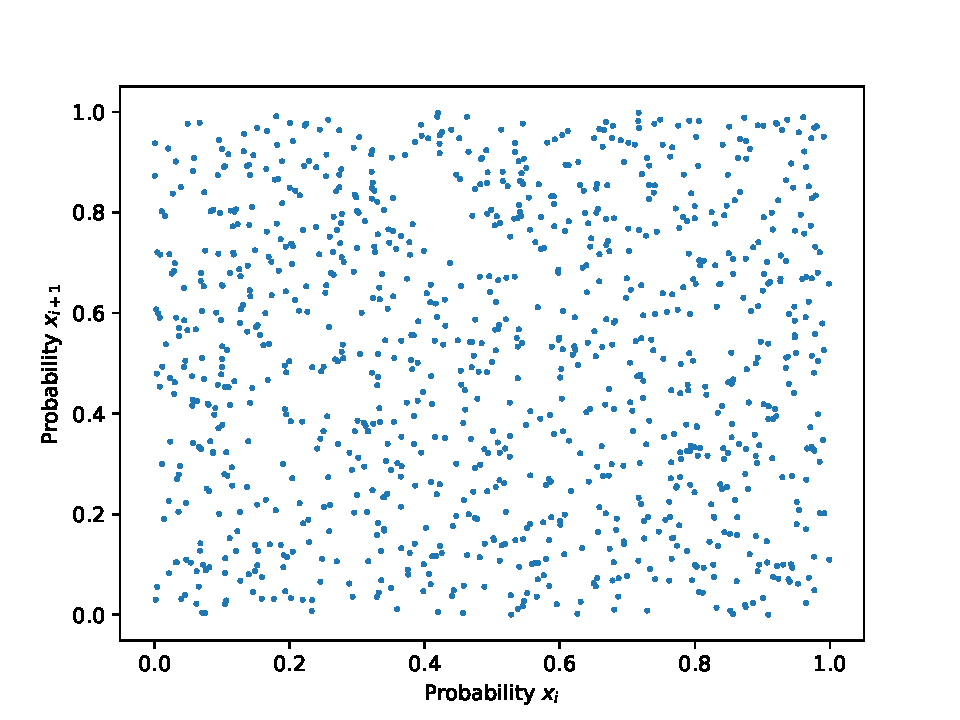
\includegraphics[width=12cm, height=7.5cm]{./Plots/1_plot_against.pdf}
\caption{TODO}
\end{figure}

\begin{figure}[!hb]
\centering
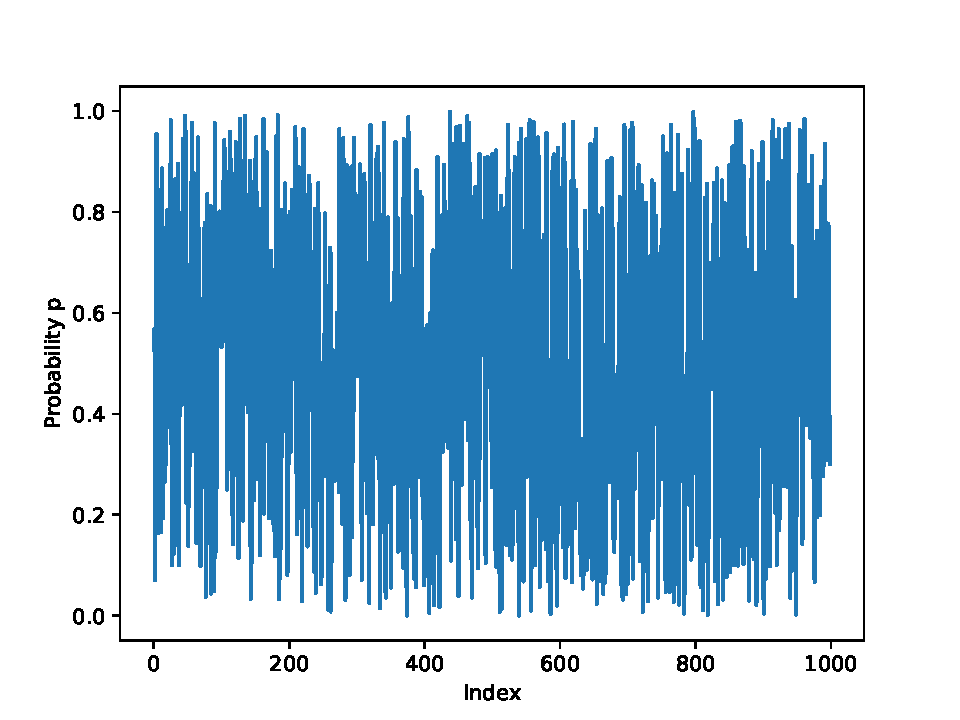
\includegraphics[width=12cm, height=7.5cm]{./Plots/1_plot_index.pdf}
\caption{TODO}
\end{figure}

\newpage
\begin{figure}[!ht]
\centering
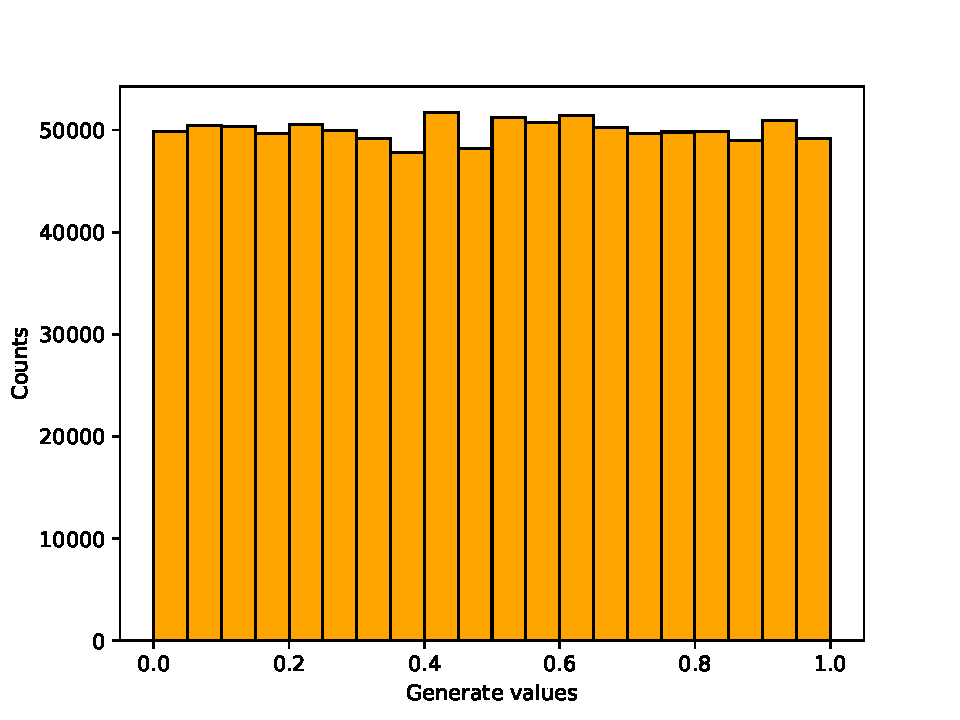
\includegraphics[width=12cm, height=7.5cm]{./Plots/1_hist_uniformnes.pdf}
\caption{TODO}
\end{figure}
\end{quote}


%\textbf{Code - helper } 
%\begin{quote}
%The code for the Poisson distribution and the factorial function.  
%\lstinputlisting[firstline=2,lastline=46]{./code/mathlib/utils.py}
%\end{quote}


%\textbf{Output}
%\begin{quote}
%The output produced by \textsf{/code/assigment1\_ a.py} 
%\lstinputlisting{./output/assigment1_a_out.txt}
%\end{quote}














\subsection*{\textbf{Question 1.b)}}
\begin{quote}

\textbf{Problem}
\begin{quote}Now use the Box-Muller method to generate 1000 normally-distributed random numbers. To check if they are following the expected Gaussian distribution, make a histogram (scaled appropriate) with the corresponding true probability distribution (normalized to integrate to 1) as line. This plot should contain the interval of -5$\sigma$ until $5\sigma$ from the theoretical probability distribution. Indicate the theoretical $1\sigma$, $2\sigma$, $3\sigma$ and $4\sigma$ interval with a line. For this plot, use $\mu =3$ and $\sigma = 2.4$ and choose bins that are appropriate.
\end{quote}

\textbf{Solution} 



\begin{quote}
The solution consists of deriving the  transformation of two i.i.d uniform variables to two i.i.d normal distributed variables with the Box-Muller method. A brief version of the derivation can be found below. The final transformation, equation \ref{EQ:boxmuller}, is  implemented in the random number generator and used to generate the plot. The final histogram is created with 20 bins and can be found on page \pageref{fig:normal}.
\\


Let $X, Y \sim G(\mu, \sigma ^2)$ be two i.i.d Gaussian distributed random variables. Their joined CDF is then given by, 
\begin{equation}
P(X \leq x_1, Y \leq y_1) =  \int_{-\infty}^{x_1} \int_{-\infty}^{y_1} G(x| \mu, \sigma^2) G(y| \mu, \sigma^2) dx dy
\end{equation}

Transforming to polar coordinates by substituting $ (x-\mu) = r \cos(\theta)$ and $ (y-\mu) = r\sin(\theta)$ yields,

\begin{align*}
P(R \leq r_1, \Theta \leq \theta_1) &= \int_0^{r_1} \int_{0}^{\theta_1} G(r\cos(\theta) \sigma + \mu| \mu, \sigma^2) G(r\sin(\theta) \sigma + \mu| \mu, \sigma^2) r dr d\theta \\
&= \frac{1}{2 \pi \sigma^2} \int_0^{r_1} \int_{0}^{\theta_1} re^{ -\frac{1}{2} \left[ \left( \frac{r\cos(\theta)}{\sigma} \right)^2  + \left( \frac{r\sin(\theta)}{\sigma} \right)^2 \right]}  dr d\theta \\
&=  \frac{1}{2 \pi \sigma^2} \int_0^{r_1} \int_{0}^{\theta_1} re^{ -\frac{r^2}{2 \sigma ^2} } dr d\theta
\end{align*}

The CDF's  for the polar coordinates are now given by, % $R$ and $\theta$ are now given by, 

\begin{align}
P(R \leq r_1) &= \frac{1}{\sigma^2} \int_{0}^{r_1}  re^{ -\frac{r^2}{2 \sigma ^2} } dr =  \int_{0}^{r_1} \frac{d}{dr} \left( -e^{ -\frac{r^2}{2 \sigma ^2}}  \right) dr = 1 - e^{- \frac{r_1^2}{2 \sigma^2}} \\
P(\Theta \leq \theta_1) &= \frac{1}{2 \pi }  \left[ -e^{-\frac{r^2}{2 \sigma^2}} \right]^{\infty}_{0} \int_{0}^{\theta_1} d\theta = \frac{\theta_1}{2\pi}
\end{align}

The CDFs can be used to convert  two uniform distributed variables to the polar coordinates of the Gaussian distributed variables. Let $U_1, U_2 \sim U(0,1)$ be two i.i.d uniform variables. From the transformation law of probability we then must have that, %The transformation law of probability then states that,

\begin{align}
P(R \leq r_1) &= P(U_1 \leq u_1) \rightarrow  1 - e^{- \frac{r_1^2}{2\sigma^2}}  = \int_{0}^{u1} du_1 = u_1 \\
P(\Theta \leq \theta) &= P(U_2 \leq u_2) \rightarrow   \frac{\theta_1}{2\pi} = \int_{0}^{u2} du_2 = u_2 
\end{align}

The transformation from the two uniform distributed variables to the polar coordinates of the Gaussian distributed variables then becomes,

\begin{align}
r_1 &=  \sqrt{-2\sigma^2 \ln(1 - u_1)} \\
\theta_1 &= 2 \pi u_2
\end{align}

Converting back to Cartesian coordinates  yields the transformation from two i.i.d uniform distributed variables to two i.i.d Gaussian distributed variables;
\begin{align}
x_1 &= r\cos(\theta) + \mu = \sqrt{-2\sigma^2 \ln(1 - u_1)} \cos( 2 \pi u_2 ) + \mu \\
y_1 &= r\sin(\theta) + \mu = \sqrt{-2\sigma^2 \ln(1 - u_1)} \sin( 2 \pi u_2 ) + \mu
\label{EQ:boxmuller}
\end{align}
\\
\\
These above transformation are implemented in  the random number generator (see page \pageref{CODE:RNG}).  The code for the generation of the plot and the created plot can be found below. The code that generates the plot makes besides the RNG use of a function for the normal distribution in the file \texttt{./Code/mathlib/statistics.py}. This file is treated as a shared module and can be found on page 22. The called function, \texttt{normal}, can be found on line 227 in this file.


\end{quote}

\textbf{Code - Plots}

\begin{quote}
The code for generating the plots. The imports are again not explicit shown, but can be found on page 19. The shared modules can be found on pages 19 and 22. 


\lstinputlisting[firstline=68,lastline=122]{./Code/assigment_1.py}
\end{quote}


\textbf{Code - Output plot(s)}
\vspace*{-0.5cm}
\begin{quote}
\begin{figure}[!hb]
\centering
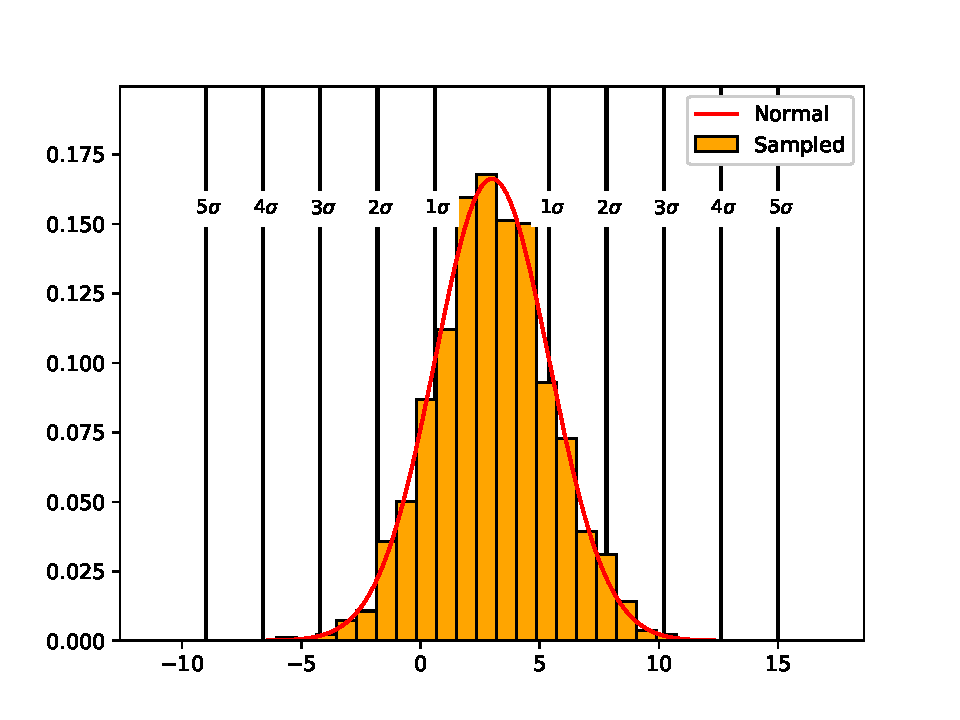
\includegraphics[width=13cm, height=7.0cm]{./Plots/1_hist_gaussian.pdf}
\caption{A histogram of the 1000 random normal distributed variables generated with the box muller method for $\mu = 3$ and $\sigma = 2.4$  (orange). The red line is the true normal distribution.  The histogram appears to approximate the distribution quite well, but displays small deviations. The bin left of the peak (the highest bin) is larger than it should be. The first bins right of the peak is smaller than it should be and the second bin right of the peak is to high.  The histogram does however still appear to be acceptable by eye. A statistical test is of course better to determine whether the histogram would truly be acceptable or not.}
\label{fig:normal}
\end{figure}
\end{quote}
\end{quote}

%\textbf{Code - output } 
%\begin{quote}
% The code that produces the output.
%\lstinputlisting{./code/assigment1_a.py}
%\end{quote}

%\textbf{Code - helper } 
%\begin{quote}
%The code for the Poisson distribution and the factorial function.  
%\lstinputlisting[firstline=2,lastline=46]{./code/mathlib/utils.py}
%\end{quote}


%\textbf{Output}
%\begin{quote}
%The output produced by \textsf{/code/assigment1\_ a.py} 
%\lstinputlisting{./output/assigment1_a_out.txt}
%\end{quote}















  







\end{document}
